\documentclass[tikz,border=2pt]{standalone}
\usepackage{amsmath,amssymb,mathrsfs,lmodern}
\usetikzlibrary{arrows.meta,positioning,calc}
\definecolor{Ink}{HTML}{163047}
\definecolor{Teal}{HTML}{087F8C}
\definecolor{Clay}{HTML}{AD4C2B}
\begin{document}
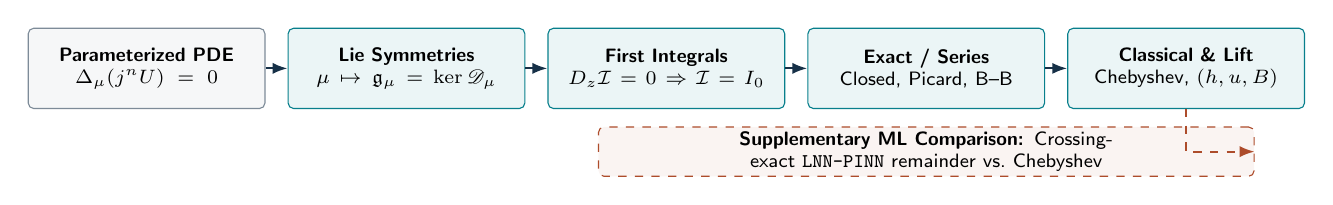
\begin{tikzpicture}[font=\sffamily\scriptsize,
  box/.style={draw=Ink!56,fill=Ink!4,rounded corners=2pt,align=center,text width=28.8mm,minimum height=10.2mm,inner sep=1.8pt},
  gate/.style={box,draw=Teal,fill=Teal!8},
  open/.style={box,draw=Clay,dashed,fill=Clay!6},
  flow/.style={-{Latex[length=1.9mm]},draw=Ink,thick}]
\node[box] (eq) {\textbf{Parameterized PDE}\\$\Delta_\mu(j^n U)=0$};
\node[gate,right=2.8mm of eq] (sym) {\textbf{Lie Symmetries}\\$\mu\mapsto\mathfrak g_\mu=\ker\mathscr D_\mu$};
\node[gate,right=2.8mm of sym] (q) {\textbf{First Integrals}\\$D_z\mathcal I=0\Rightarrow\mathcal I=I_0$};
\node[gate,right=2.8mm of q] (profile) {\textbf{Exact / Series}\\Closed, Picard, B--B};
\node[gate,right=2.8mm of profile] (lift) {\textbf{Classical \& Lift}\\Chebyshev, $(h,u,B)$};
\draw[flow] (eq)--(sym);
\draw[flow] (sym)--(q);
\draw[flow] (q)--(profile);
\draw[flow] (profile)--(lift);
\node[open,below=2.2mm of profile,xshift=0mm,text width=82mm,minimum height=5.8mm] (cor)
  {\textbf{Supplementary ML Comparison:}\enspace Crossing-exact \texttt{LNN-PINN} remainder vs.\ Chebyshev};
\draw[flow,draw=Clay,dashed] (lift.south) |- (cor.east);
\end{tikzpicture}
\end{document}
